\section{Introduction}
\label{sec:Introduction}
%wat, waar, waarom
%maatschappelijke bijdrage van het project
The environment is constantly being influenced by humanity and this influence has been debated since the hippie movement in the 60s.
The debate on the weight humanity has on the environment has also been fuelled in recent years; the full impact of oil-spills and climate change are still being debated about. \citepos

This project will focus on one of the environmental hazards: Plastic Soup.
However, the project will not focus on the problem, or how Plastic Soup affects nature, but how Artificial Intelligence can help to clean up the waste.

%Environment is important, AI can help with the conservation... [oa citeren van \citep{vannature}]


\subsection{Plastic Soup: Environmental problem}
\label{sec:Intro-Plastic Soup}
%Bede context, Maatschappelijke relevantie
%Large amounts of plastic waste ends up in the world's ocean... [oa citeren van \citep{barnes2005drifting}, \citep{moore2011plastic}]
Large amounts of plastic waste end up in the world's oceans and have a significant impact on marine life \citep{barnes2005drifting}.
Plastic Soup or Plastic Ocean are both a collective noun for this environmental problem.
As \citeauthor{barnes2005drifting} indicate, the amount of flotsam in the oceans grows annually as does the increasing proportion of plastic.

When plastic objects are disposed of in rivers, they float through rivers into the ocean.
The currents in the oceans transport the flotsam around the world to influence marine life.
In figure \ref{fig:plastic-where} the probable location of the Great Pacific Ocean Patch is shown\footnote{source: \url{http://education.nationalgeographic.com/education/encyclopedia/great-pacific-garbage-patch} }.
Because the plastic does not decay in nature, a lot of marine life ingests the plastic into their digestive system. 
Figure \ref{fig:plastic-bird} shows how much plastic can end up in a bird.

\begin{figure}[h!bt]
\centering
\ifx\showfig\undefined
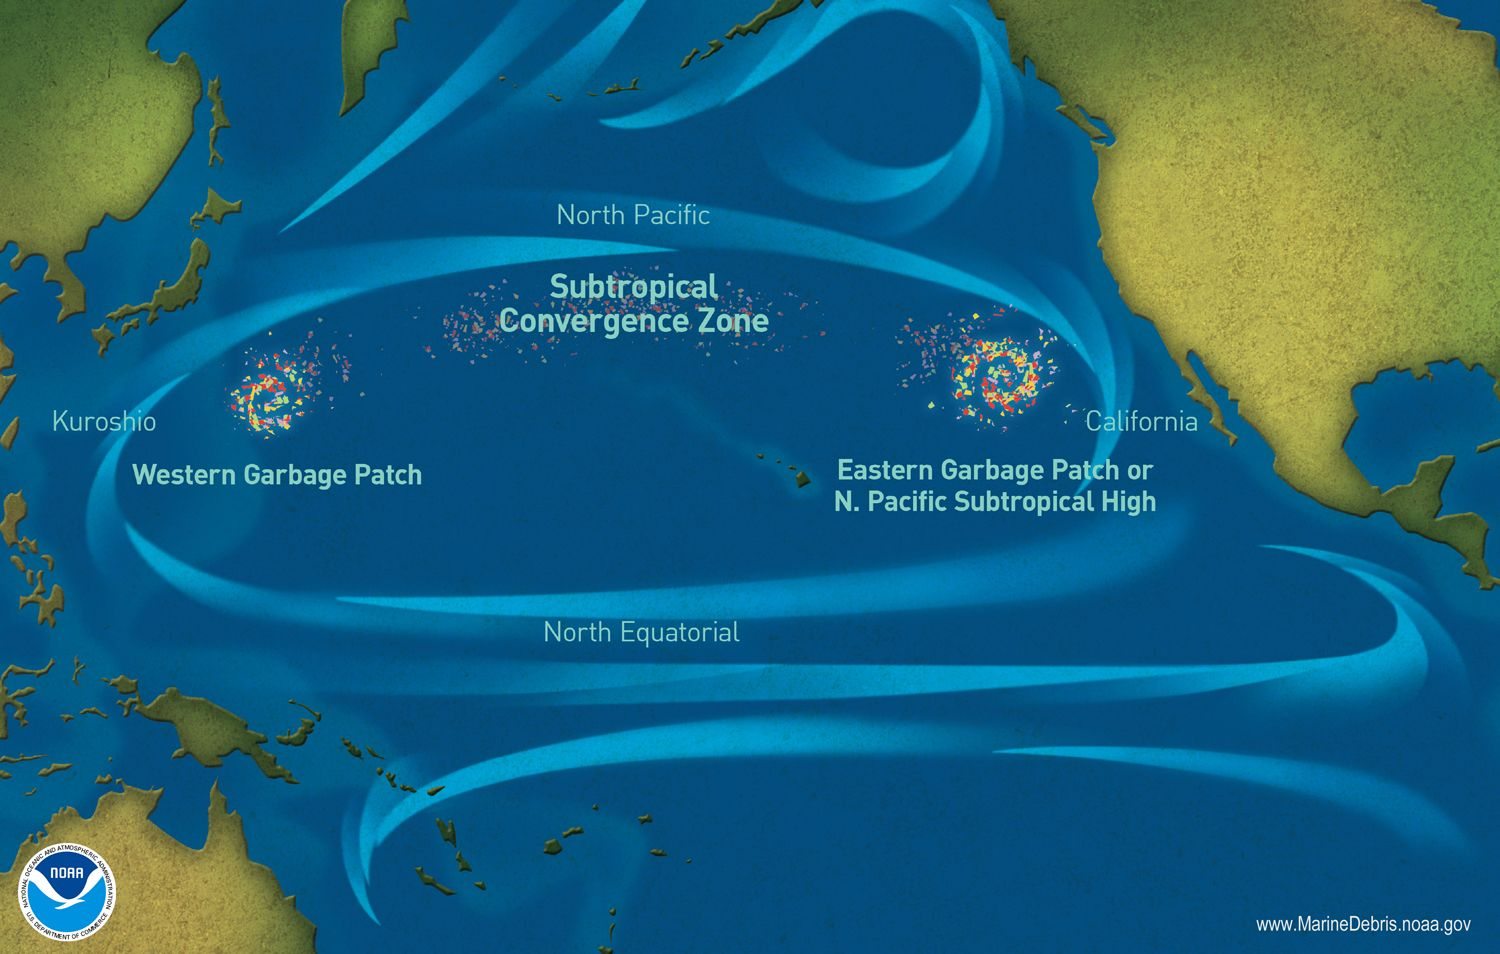
\includegraphics[keepaspectratio=true,width=.8\textwidth]{images/garbage-patch.jpg} \fi
\caption{Ocean currents in the Pacific that `collect' the Plastic Soup. Map by NOAA }
\label{fig:plastic-where}
\end{figure}

\begin{figure}[h!bt]
\centerline{
\begin{minipage}{1.3\textwidth}
\begin{subfigure}[t]{.48\textwidth}
\ifx\showfig\undefined
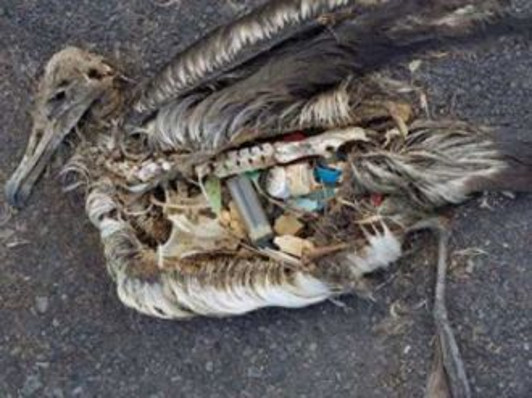
\includegraphics[keepaspectratio=true,width=\textwidth]{images/Bird_with_plastic_stomach.jpg} \fi
\caption{The stomach contents of a bird that ate plastic. Photograph by Chris Jordan, U.S. Fish and Wildlife Service }
\label{fig:plastic-bird}
\end{subfigure}
\hfill
\begin{subfigure}[t]{.48\textwidth}
\ifx\showfig\undefined
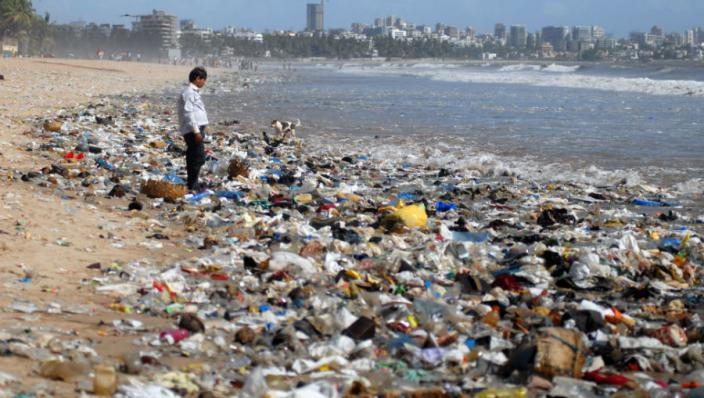
\includegraphics[keepaspectratio=true,width=\textwidth]{images/plastic-beach.jpg} \fi
\caption{A polluted beach in Mumbai, India. Photograph by EPA }
\label{fig:plastic-beach}
\end{subfigure}
\caption{Impact of Plastic Soup on the environment and society}
\label{fig:plastic-impact}
\end{minipage}
}
\end{figure}

In addition to the dangers for marine life, large amounts of plastic end up on beaches, as shown in figure \ref{fig:plastic-beach}.
This has a sizeable impact on the 

The most significant problem is probably micro-plastic.
When plastic floats in water for some time, sunlight and minerals break the plastic objects down into grains.
These grains of plastic are usually several micro meters in size and can infect the ecosystem to a large extend \citet{moore2011plastic}.

The weight of Plastic Soup on the environment has caused several organisations to form in order to address this problem and find solutions to the problem.
The nascency of organisations addressing the problem and searching for solutions has gained media attention and thus cause the growing awareness for the Plastic Soup.

These organisations would benefit with systems that can detect plastic automatically.
Therefore, this project will focus on techniques that are able to distinguish plastic from marine life in ocean water.

\subsection{Project outline}
\label{sec:Intro-Me}
%Onderzoeksvraag, proefopzet, hypothese
To develop a system that can detect plastic, state-of-the-art imaging techniques will be used.
In recent years the accuracy of imaging techniques on object recognition have been growing, as section \ref{sec:Theory-CV} describes.
This project will research how these techniques will perform on Plastic Soup detection.

A dataset of annotated images has been constructed to be used in this project.
This dataset can be used to train and test the algorithm.
To recognise the plastic containing images, a Convolutional Neural Network (CNN) will be used.
The CNN will not be trained on the data itself, however a pre-trained network will be used to construct a feature-vector of the image.
These feature-vectors will be used to train a classifier to classify the images in ether containing or not containing plastic.
The classifier used in this project is a Support Vector Machine (SVM); to distinguish between plastic and marine-life, two SMVs will be trained.

This method for image recognition should give an appropriate baseline.
\todo{uitbreiden}

\subsection{Outline of the thesis chapters}
\label{sec:Intro-Outline}
The performance of the plastic-soup detector made in this project are described in section \ref{sec:Conclusion} from the results in section \ref{sec:Results}.
In section \ref{sec:Method} the method of the project is shown, and in section \ref{sec:Discussion} I will go into the parts that can be improved in further research.
But first, in section \ref{sec:Theory} the current state-of-the-art techniques in the field of Computer Vision.
%In section \ref{sec:Theory}... \todo{when the thesis is finished, fill this paragraph}















\iffalse
%...dangers of microplastic...

%...big impact on marine life and life in general...

%==Urgentie had groter kunnen worden gemaakt. Hoeveel plastic is er? Wat wordt er al aan gedaan? Hoeveel vogels hebben er last van? Waar komt dat plastic vandaan? Etc.

\subsection{Current solutions}
\label{sec:Intro-Current}


One of the organisations that addresses the problem is Saraswater \citeneed.
This organisation is developing techniques to clean the ocean of this plastic waste.
Saraswater made an apparatus that can be mounted on a ship which shovel the waste from the water.
The small scale experiments that they performed show promising results.

These plastic shovelling ships would benefit from being autonomous.
If no humans are needed, the ships can roam the oceans for many months without the need for visiting harbours.

%One of them is Saraswater. They are developing techniques .. [oa bronnen van de organisaties (niet zozeer artikelen)]
%To help she ships of saraswater, atomise the process with autonomous agents...
%laatse zin: dit is niet genoeg, automatiseering
\subsection{Automation}
\label{sec:Intro-Automate}
When the ships are controlled by an autonomous agent, less human labour is needed for the clean up of the Plastic Ocean.
This project will try to begin with automation of the clean-up.

The automation of the ships is a long term goal.
Before the ships of Saraswater can be autonomous, they first need to `see' to know where the plastic is to clean up.
That is why this project will focus on detecting plastic in ocean water from image data.
Further research expanding this project could develop true autonomous agents controlling the plastic shovelling ships.



%Using state-of-the-art imaging techniques... probably effect... Investigate what will work best by using different algorithms on a dataset of annotated images...


\fi